\section{Synchronizace dat s VCS}
Tato podkapitola je věnována implementaci mechanismu synchronizace dat se systémy pro správu verzí softwaru. Tento modul představuje klíčovou komponentu pro získávání metrik o aktivitě vývojářů, jež jsou následně zpracovávány a vizualizovány uživatelům. Přestože je primárním cílem integrace platforem GitHub a GitLab, architektura byla navržena s ohledem na možnou budoucí rozšiřitelnost o další poskytovatele.

\subsection{Architektura řešení}
Pro zajištění modularity a snadné udržovatelnosti kódu byl při návrhu synchronizačního procesu kladen důraz na abstrakci. V rámci hlavní logiky aplikace nejsou využívána přímá volání specifických API jednotlivých služeb, ale komunikace je realizována výhradně prostřednictvím definovaných rozhraní.

\dirtree{%
  .1 .
  .1 Drivers\DTcomment{složka s podporovanými VCS}.
    .2 GitHub.
      .3 GitHubAuthenticator.php\DTcomment{zajišťuje autentizaci požadavku}.
      .3 GitHubMapper.php\DTcomment{mapuje výsledky GraphQL dotazů na DTO}.
      .3 GitHubProviderFactory.php\DTcomment{vytváří GitProvider instanci}.
      .3 GitHubQueryRepository.php\DTcomment{obsahuje GraphQL dotazy}.
    .2 GitLab\DTcomment{obsahuje typově stejné soubory jako složka GitHub}.
  .1 Interfaces\DTcomment{rozhraní, která musí každý VCS implementovat}.
    .2 Authenticator.php.
    .2 Mapper.php.
    .2 QueryRepository.php.
  .1 GitProvider.php\DTcomment{obsahuje hlavní logiku pro synchronizaci}.
  .1 GitProviderFactory.php\DTcomment{factory}.
}

\vspace{10pt}

Jak je patrné z výše uvedené adresářové struktury, ve složce \texttt{Drivers} jsou umístěny konkrétní implementace pro služby GitHub a GitLab. Vztah mezi jednotlivými třídami a rozhraními, který je založen na aplikaci návrhového vzoru Strategy, je schematicky znázorněn na obrázku \ref{figure:strategy-pattern}. Díky tomuto přístupu v kombinaci se vzorem Factory není systém pevně vázán na konkrétní systém pro správu verzí. Případné budoucí rozšíření o nového poskytovatele by vyžadovalo pouze implementaci příslušného driveru splňujícího předepsaná rozhraní, a to bez nutnosti zásahu do existující logiky synchronizace.

\begin{figure}[h]
    \caption{Využití návrhového vzoru Strategy při získávání dat z VCS}
    \label{figure:strategy-pattern}
    \centering
    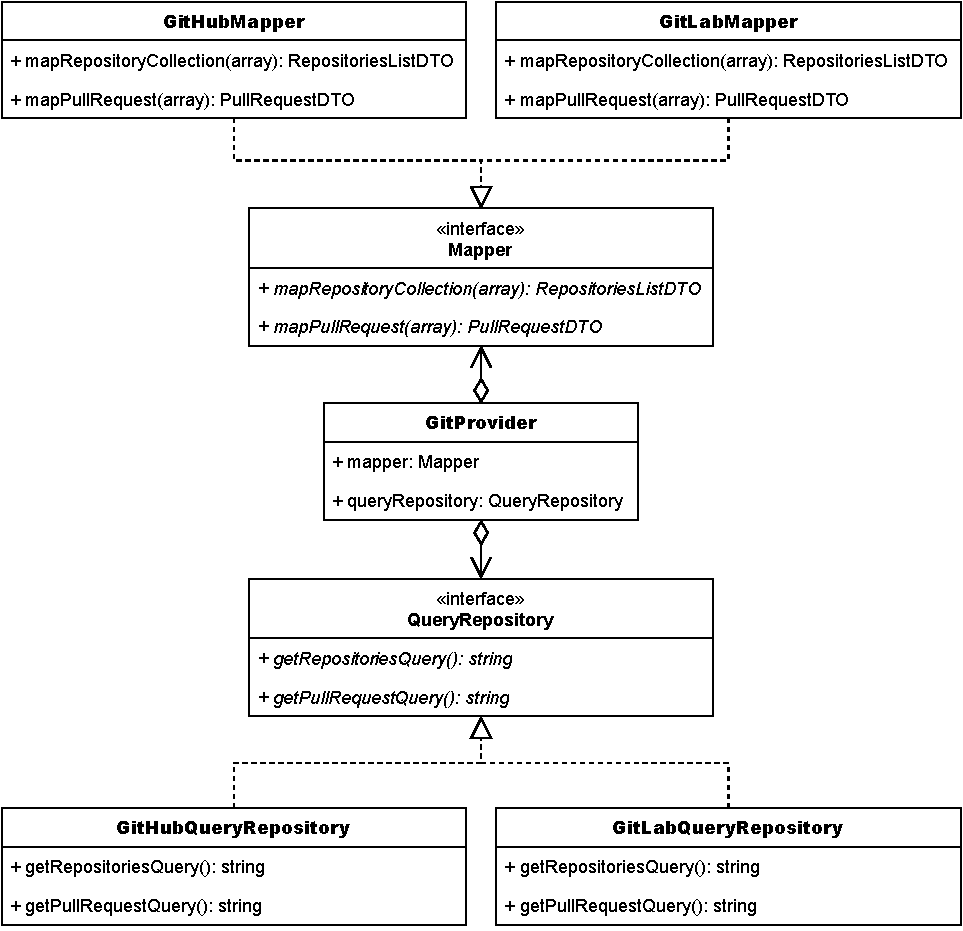
\includegraphics[width=0.98\linewidth]{images/strategy-pattern.pdf}
\end{figure}

Samotný proces získávání dat je realizován v definované posloupnosti kroků, která využívá výše popsané komponenty. Nejprve je požadavek autentizován prostřednictvím komponenty \texttt{Authenticator}. Následně je z \texttt{QueryRepository} získán konkrétní GraphQL dotaz a je provedeno samotné vykonání požadavku vůči API poskytovatele. V závěrečné fázi je výsledek dotazu transformován pomocí komponenty \texttt{Mapper} na DTO, se kterým aplikace dále pracuje.

\subsection{Autentizace požadavku}
Pro autentizaci požadavků vůči platformám GitHub a GitLab je využívána HTTP hlavička \texttt{Authorization}, která je součástí každého odchozího volání. Z bezpečnostních důvodů je doporučen aplikovat princip minimálních oprávnění, kdy je přístup omezen výhradně na čtení dat nezbytných pro sběr metrik. Tímto opatřením je minimalizováno riziko zneužití v případě potenciálního úniku přístupových údajů.

\subsubsection{GitHub}
Pro autentizaci požadavků u platformy GitHub byla zvolena metoda prostřednictvím GitHub App. Privátní klíč, nezbytný pro generování instalačních tokenů, je uložen v konfiguračním souboru \texttt{.env}, který není součástí verzovacího systému. Vzhledem k hodinové platnosti instalačních tokenů je implementován mechanismus jejich ukládání do mezipaměti. K obnově dochází až po vypršení platnosti, čímž je efektivně redukován počet nutných volání API pro autentizaci. Konfigurace GitHub App vyžaduje nastavení oprávnění \texttt{Repository permissions – Pull requests} v režimu \texttt{Read-only}.

\subsubsection{GitLab}
V případě platformy GitLab byl pro autentizaci zvolen přístup prostřednictvím přístupových tokenů. S ohledem na nižší implementační složitost byla tato metoda upřednostněna před komplexnějším řešením využívajícím protokol OAuth 2.0. Pro zajištění korektní synchronizace dat je u tokenu vyžadován rozsah oprávnění \texttt{read\_api}. Samotné tokeny jsou v databázi aplikace uchovávány v šifrované podobě.

\subsection{Proces synchronizace a plánování úloh}
